\documentclass[12pt,a4paper]{article}
\usepackage[utf8]{inputenc}
\usepackage[T1]{fontenc}
\usepackage[english]{babel}
\usepackage{geometry}
\usepackage{booktabs}
\usepackage{longtable}
\usepackage{array}
\usepackage{xcolor}
\usepackage{colortbl}
\usepackage{graphicx}
\usepackage{fancyhdr}
\usepackage{titlesec}
\usepackage{tikz}
\usepackage{enumitem}
\usepackage{hyperref}
\usepackage{multicol}
\usepackage{listings}
\usepackage{tcolorbox}
\usepackage{amssymb}
\usepackage{amsmath}
\usepackage{float}


\geometry{margin=2cm}
\pagestyle{fancy}
\fancyhf{}
\rhead{Machine Learning Project}
\lhead{Customer Behavioral Analysis}
\rfoot{Page \thepage}

% Custom colors
\definecolor{headerblue}{RGB}{41, 65, 114}
\definecolor{lightgray}{RGB}{245, 245, 245}
\definecolor{accentorange}{RGB}{230, 126, 34}
\definecolor{codegreen}{RGB}{0,128,0}
\definecolor{codegray}{RGB}{128,128,128}
\definecolor{codepurple}{RGB}{128,0,128}
\definecolor{backcolour}{RGB}{248,248,248}
\definecolor{warningred}{RGB}{231, 76, 60}
\definecolor{successgreen}{RGB}{46, 204, 113}

\lstdefinestyle{mystyle}{
    backgroundcolor=\color{backcolour},
    commentstyle=\color{codegreen},
    keywordstyle=\color{codepurple},
    numberstyle=\tiny\color{codegray},
    stringstyle=\color{codegreen},
    basicstyle=\ttfamily\footnotesize,
    breakatwhitespace=false,
    breaklines=true,
    captionpos=b,
    keepspaces=true,
    numbers=left,
    numbersep=5pt,
    showspaces=false,
    showstringspaces=false,
    showtabs=false,
    tabsize=2
}
\lstset{style=mystyle}


\tcbset{
    colback=backcolour,
    colframe=headerblue,
    fonttitle=\bfseries,
    boxrule=1pt,
    arc=3mm
}


\titleformat{\section}
{\normalfont\Large\bfseries}
{\thesection}{1em}{}[{\titlerule[2pt]}]

\titleformat{\subsection}
{\normalfont\large\bfseries}
{\thesubsection}{1em}{}

% Custom column definitions
\newcolumntype{C}[1]{>{\centering\arraybackslash}p{#1}}
\newcolumntype{L}[1]{>{\raggedright\arraybackslash}p{#1}}

\begin{document}


\begin{titlepage}
\vspace{2cm}

\begin{center}
{\Huge\textbf{Machine Learning Project}}\par
\vspace{0.5cm}
{\Large\textit{Retail Customer Behavioral Analysis}}\par

\vspace{4cm}

{\LARGE\textbf{REPORT}}\par
\vspace{1cm}
{\large Project: Gift E-commerce}\par
\vspace{2cm}
{\large \textbf{Prepared by Haythem FRIKHA}}
\vspace{3cm}

\rule{10cm}{2pt}

\vspace{5cm}

{\textbf{Academic Year: 2025-2026}}

\end{center}
\vfill
\end{titlepage}

\tableofcontents
\newpage

%==============================================================================
\section{Introduction}
%==============================================================================

This report presents the work carried out during the Machine Learning workshop on customer behavioral analysis for a gift-focused e-commerce store. The main objective of this project is to develop machine learning solutions that can:

\begin{itemize}
    \item \textbf{Personalize the marketing strategy} through customer segmentation
    \item \textbf{Reduce churn rate} with predictive modeling
    \item \textbf{Increase revenue} by targeting at-risk customers
\end{itemize}

The provided dataset contains \textbf{4,372 customers} described by \textbf{52 variables}, including RFM metrics (Recency, Frequency, Monetary), demographic data, purchasing behavior, and account information.

%==============================================================================
\subsection{Project Architecture}
%==============================================================================

A well-structured software architecture is essential for maintainability, reproducibility, and deployment of Machine Learning solutions. This subsection describes the project directory structure.

\subsubsection{Directory Structure}

The project follows a standard data science layout, clearly separating raw data, processed data, code, models, and outputs.

\begin{lstlisting}[language=bash]
ml-retail/
|-- data/
|   |-- raw/                    # Raw data
|   |-- processed/              # Cleaned data
|   |-- train_test/             # Train/test splits
|-- models/                     # Trained models
|-- reports/                    # Visualizations
|-- src/                        # Source code
    |-- preprocessing.py        # Preprocessing pipeline
    |-- train_model.py          # Model training
    |-- segmentation.py         # Customer segmentation
    |-- predict.py              # Prediction script
    |-- utils.py                # Utility functions
\end{lstlisting}

%==============================================================================
\section{Data Preprocessing}
%==============================================================================

Preprocessing is a critical step to ensure model quality. We implemented a complete pipeline in the file \texttt{src/preprocessing.py}.

\subsection{Handling Missing Values}

Several strategies were used to handle missing values depending on each variable's nature.

\subsubsection{Age Variable}
The \texttt{Age} variable contained \textbf{1,311 missing values} (29.99\% of the dataset). We used \textbf{K-Nearest Neighbors (KNN)} imputation with the following parameters:
\begin{itemize}
    \item Number of neighbors: $k = 5$
    \item Inverse-distance weighting
    \item Variables used: Recency, Frequency, MonetaryTotal, MonetaryAvg, CustomerTenureDays, FirstPurchaseDaysAgo
\end{itemize}

This approach captures correlations between age and purchasing behavior, producing more realistic imputations than a simple mean or median.

\subsubsection{AvgDaysBetweenPurchases Variable}
This variable had \textbf{79 missing values}, imputed using the median (1.15 days).

\subsection{Outlier and Sentinel Value Processing}

Some variables contained \textbf{sentinel values} used to encode missing data or errors:

\begin{table}[H]
\centering
\begin{tabular}{lll}
\toprule
\textbf{Variable} & \textbf{Anomalous values} & \textbf{Occurrence count} \\
\midrule
SupportTicketsCount & -1, 999 & 130 (2.97\%) \\
SatisfactionScore & -1, 0, 99 & 349 (7.98\%) \\
\bottomrule
\end{tabular}
\caption{Identified and corrected sentinel values}
\end{table}

These values were replaced by each variable's median and then clipped to valid ranges (0-15 for SupportTicketsCount, 1-5 for SatisfactionScore).

\subsection{Feature Engineering}

To improve predictive performance, we created additional features from raw data.

\subsubsection{Registration Date}
The \texttt{RegistrationDate} variable was parsed and split into four new variables:
\begin{itemize}
    \item \texttt{RegYear}: Registration year
    \item \texttt{RegMonth}: Registration month
    \item \texttt{RegDay}: Registration day
    \item \texttt{RegWeekday}: Day of week (0=Monday, 6=Sunday)
\end{itemize}

\subsubsection{IP Address}
From the \texttt{LastLoginIP} variable, we extracted:
\begin{itemize}
    \item \texttt{IsPrivateIP}: Boolean flag (326 customers with private IPs)
    \item \texttt{LoginCountry}: Login country (using the DB-IP Lite database)
\end{itemize}

The login country distribution shows a mostly US customer base (1,494 customers), followed by China (362) and Japan (219).

\subsection{Removing Unreliable Variables}

Some variables were excluded from preprocessing due to questionable reliability.

The variable \texttt{NewsletterSubscribed} was removed because it was marked as unreliable in the project documentation.

%==============================================================================
\section{Data Leakage Detection and Correction}
%==============================================================================

A detailed analysis of correlations between features and the \texttt{Churn} target revealed several cases of \textbf{data leakage}, which would have compromised model validity.

\subsection{Excluded Variables}

The following table summarizes the removed variables and why they were excluded.

\begin{table}[H]
\centering
\begin{tabular}{L{3.5cm}L{9cm}}
\toprule
\textbf{Variable} & \textbf{Reason for exclusion} \\
\midrule
ChurnRiskCategory & Directly derived from the target variable (100\% correlation) \\
RFMSegment & The "Dormants" category corresponds to 100\% churned customers \\
CustomerType & The "Lost" category corresponds to 100\% churned customers \\
Recency & Perfect split: Churn=0 if Recency $\leq$ 90 days, Churn=1 if Recency $>$ 90 days \\
\bottomrule
\end{tabular}
\caption{Variables removed due to data leakage}
\end{table}

\subsection{Recency Variable Analysis}

The analysis showed that \texttt{Recency} itself defines churn:
\begin{itemize}
    \item Non-churned customers: Recency $\in [1, 90]$ days
    \item Churned customers: Recency $\in [91, 374]$ days
\end{itemize}

This finding is critical: churn is effectively defined as inactivity for more than 90 days. Using this feature would amount to predicting the past with the past.

%==============================================================================
\section{Predictive Churn Modeling}
%==============================================================================

This section details the process used to build and evaluate classification models for churn prediction. Several approaches were implemented, from preprocessing to comparison of seven different algorithms.

\subsection{Data Preparation for Modeling}

Before training the models, we applied several essential data transformations.

\subsubsection{Feature Encoding}
\begin{itemize}
    \item \textbf{Numeric variables (35)}: Standardized using \texttt{StandardScaler}
    \item \textbf{Categorical variables (14)}: One-hot encoded using \texttt{OneHotEncoder}
\end{itemize}

\subsubsection{Train/Test Split}
The dataset was split into:
\begin{itemize}
    \item \textbf{Training set}: 3,497 samples (80\%)
    \item \textbf{Test set}: 875 samples (20\%)
\end{itemize}

Stratification was applied to preserve target distribution (33.26\% churn) in both sets.

\subsubsection{Class Imbalance Handling}

A churn rate of 33.26\% represents moderate class imbalance. We applied \textbf{SMOTE} (Synthetic Minority Over-sampling Technique) on the training set:
\begin{itemize}
    \item Before SMOTE: 2,334 non-churned, 1,163 churned
    \item After SMOTE: 2,334 non-churned, 2,334 churned
\end{itemize}

\subsection{Evaluated Models}

Seven classification algorithms were trained and compared:

\begin{table}[H]
\centering
\begin{tabular}{lccccc}
\toprule
\textbf{Model} & \textbf{Accuracy} & \textbf{Precision} & \textbf{Recall} & \textbf{F1} & \textbf{ROC-AUC} \\
\midrule
\textbf{XGBoost (Tuned)} & \textbf{99.1\%} & \textbf{99.0\%} & \textbf{98.3\%} & \textbf{98.6\%} & \textbf{99.97\%} \\
Logistic Regression & 98.4\% & 98.6\% & 96.6\% & 97.6\% & 99.8\% \\
Gradient Boosting & 98.3\% & 96.9\% & 97.9\% & 97.4\% & 99.9\% \\
Decision Tree & 97.3\% & 94.9\% & 96.9\% & 95.9\% & 97.2\% \\
SVM & 97.1\% & 98.9\% & 92.4\% & 95.6\% & 99.7\% \\
Random Forest & 94.9\% & 96.6\% & 87.6\% & 91.9\% & 98.7\% \\
KNN & 84.1\% & 70.9\% & 88.7\% & 78.8\% & 92.5\% \\
\bottomrule
\end{tabular}
\caption{Model performance comparison on the test set}
\end{table}

\subsection{Hyperparameter Optimization}

To further improve the best-performing model, XGBoost (selected based on F1 score), we performed hyperparameter tuning with \textbf{GridSearchCV} and 5-fold cross-validation.

\begin{tcolorbox}[title=Optimal Hyperparameters - XGBoost, colback=white, colframe=black]
\begin{itemize}
    \item \texttt{learning\_rate}: 0.1
    \item \texttt{max\_depth}: 7
    \item \texttt{n\_estimators}: 100
    \item \texttt{subsample}: 0.8
\end{itemize}
Cross-validation F1 score: 99.09\%
\end{tcolorbox}

\subsection{Feature Importance}

Understanding which factors drive model predictions is essential for interpretability and actionability. XGBoost feature importance highlights the strongest churn predictors:

\begin{enumerate}
    \item \textbf{LoyaltyLevel\_Établi} (35.3\%): Established customers are significantly less likely to churn
    \item \textbf{FavoriteSeason\_Hiver} (20.4\%): Seasonal buying patterns are highly predictive
    \item \textbf{PreferredMonth} (20.0\%): Preferred purchase month indicates engagement level
    \item \textbf{LoyaltyLevel\_Nouveau} (5.8\%): New customers show distinct behavioral patterns
    \item \textbf{CustomerTenureDays} (4.5\%): Customer tenure
\end{enumerate}

%==============================================================================
\section{Customer Segmentation}
%==============================================================================

In addition to churn prediction, a complementary customer segmentation approach was developed. This RFM analysis supports personalized marketing strategies and helps identify customer groups with distinct characteristics and needs.

\subsection{Methodology}

Segmentation was performed using a quantitative approach based on the K-Means algorithm.

\subsubsection{RFM Variables}
\begin{itemize}
    \item \textbf{Recency}: Number of days since the last purchase
    \item \textbf{Frequency}: Total number of purchases
    \item \textbf{Monetary}: Total amount spent
\end{itemize}

\subsubsection{Clustering Algorithm}
We used \textbf{K-Means} with the following steps:
\begin{enumerate}
    \item Standardization of RFM variables using \texttt{StandardScaler}
    \item Search for the optimal number of clusters using silhouette score
    \item Application of K-Means with $k=3$ clusters
\end{enumerate}

\subsection{Identified Segments}

Running K-Means revealed three distinct segments with very different RFM profiles and churn rates.

\begin{table}[H]
\centering
\begin{tabular}{L{3cm}ccccc}
\toprule
\textbf{Segment} & \textbf{Customers} & \textbf{Churn Rate} & \textbf{Avg. Recency} & \textbf{Avg. Freq.} & \textbf{Avg. Amount} \\
\midrule
At Risk & 1,109 (25.4\%) & 100\% & 246 days & 1.85 & 460 \$ \\
Champions & 26 (0.6\%) & 0\% & 6 days & 83.35 & 75,966 \$ \\
Active Customers & 3,237 (74.0\%) & 11\% & 40 days & 5.55 & 1,796 \$ \\
\bottomrule
\end{tabular}
\caption{Profile of identified customer segments}
\end{table}

\subsection{Segment-Based Marketing Recommendations}

To maximize the effectiveness of marketing interventions, specific recommendations were defined for each segment.

\begin{tcolorbox}[title=Champions Segment (Priority: HIGH VALUE), colback=white, colframe=black]
\textbf{Recommended actions:}
\begin{itemize}
    \item Exclusive offers and early access to new products
    \item Loyalty program with VIP benefits
    \item Review requests and referral program
    \item Personalized thank-you communications
\end{itemize}
\textbf{Channels:} Email, Direct mail, Dedicated account manager
\end{tcolorbox}

\begin{tcolorbox}[title=At-Risk Segment (Priority: URGENT), colback=white, colframe=black]
\textbf{Recommended actions:}
\begin{itemize}
    \item Win-back campaign with special discounts
    \item Survey to understand inactivity drivers
    \item Personalized "We miss you" messages
    \item Time-limited exclusive offers
\end{itemize}
\textbf{Channels:} Email, SMS, Direct mail
\end{tcolorbox}

\begin{tcolorbox}[title=Active Customers Segment (Priority: MEDIUM), colback=white, colframe=black]
\textbf{Recommended actions:}
\begin{itemize}
    \item Upselling toward higher-value products
    \item Cross-selling complementary products
    \item Free-shipping thresholds to increase basket size
    \item Early access to seasonal sales
\end{itemize}
\textbf{Channels:} Email, Retargeting ads
\end{tcolorbox}

%==============================================================================
\section{Generated Visualizations}
%==============================================================================

The project produces six key visualizations stored in the \texttt{reports/} directory. Each chart provides critical insights into model performance and customer behavior, covering model comparison, predictive evaluation, and segment analysis.

\subsection{Model Comparison}

This visualization includes two side-by-side bar charts for fast comparison of the seven algorithms:
\begin{itemize}
    \item \textbf{Left panel}: Classification metrics (Accuracy, Precision, Recall, F1) for each model
    \item \textbf{Right panel}: ROC-AUC score per model
\end{itemize}

It quickly identifies XGBoost as the top-performing model across all criteria.

\begin{figure}[H]
\centering
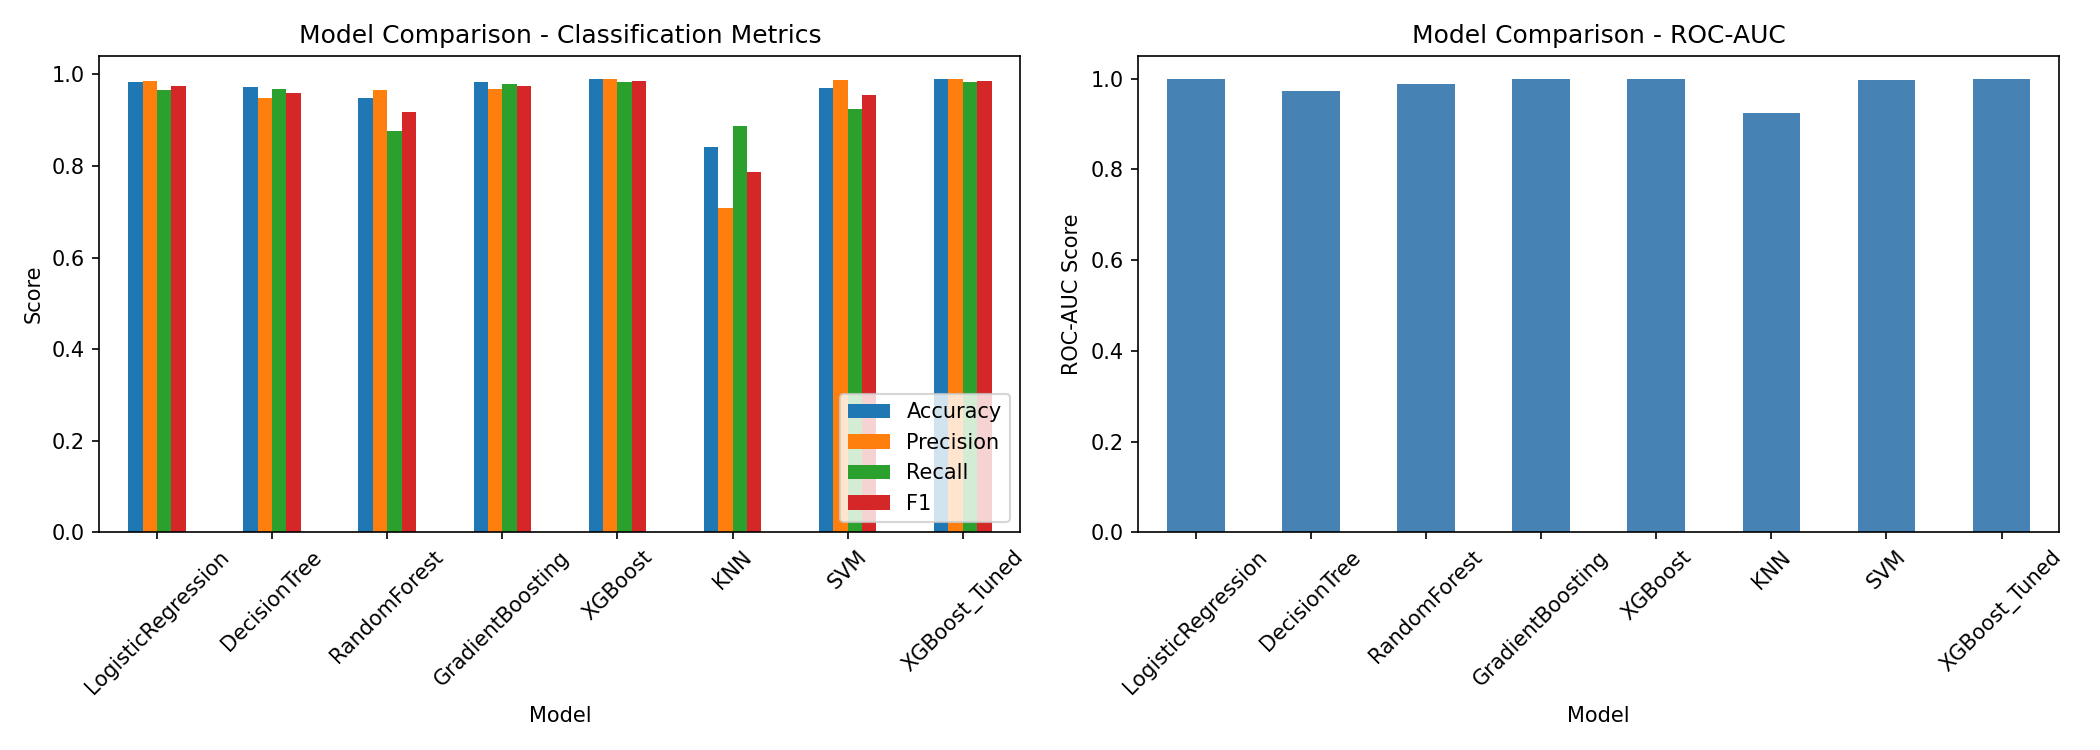
\includegraphics[width=\textwidth]{model_comparison.png}
\caption{Visual comparison of the seven models across classification metrics and ROC-AUC.}
\label{fig:model_comparison}
\end{figure}

\subsection{ROC Curves}

Beyond core metrics, a deeper view of each model's discrimination capability is needed. ROC curves display all models on the same plot:
\begin{itemize}
    \item X-axis: False Positive Rate (FPR)
    \item Y-axis: True Positive Rate (TPR)
    \item The diagonal line represents a random classifier (AUC = 0.5)
\end{itemize}

Curves closer to the top-left corner indicate better performance.

\subsection{Confusion Matrix}

For a granular understanding of classification errors made by the best model, a detailed confusion matrix is generated. It presents XGBoost predictions as a heatmap:
\begin{itemize}
    \item \textbf{True Negatives (TN)}: Customers correctly identified as non-churned
    \item \textbf{True Positives (TP)}: Customers correctly identified as churned
    \item \textbf{False Positives (FP)}: Non-churned customers incorrectly flagged (Type I error)
    \item \textbf{False Negatives (FN)}: Churned customers missed by the model (Type II error)
\end{itemize}

\subsection{Feature Importance}

To understand churn drivers, feature importance analysis is essential. A horizontal bar chart shows the top 20 most influential XGBoost features, ranked by their contribution to reducing prediction error.

\begin{figure}[H]
\centering
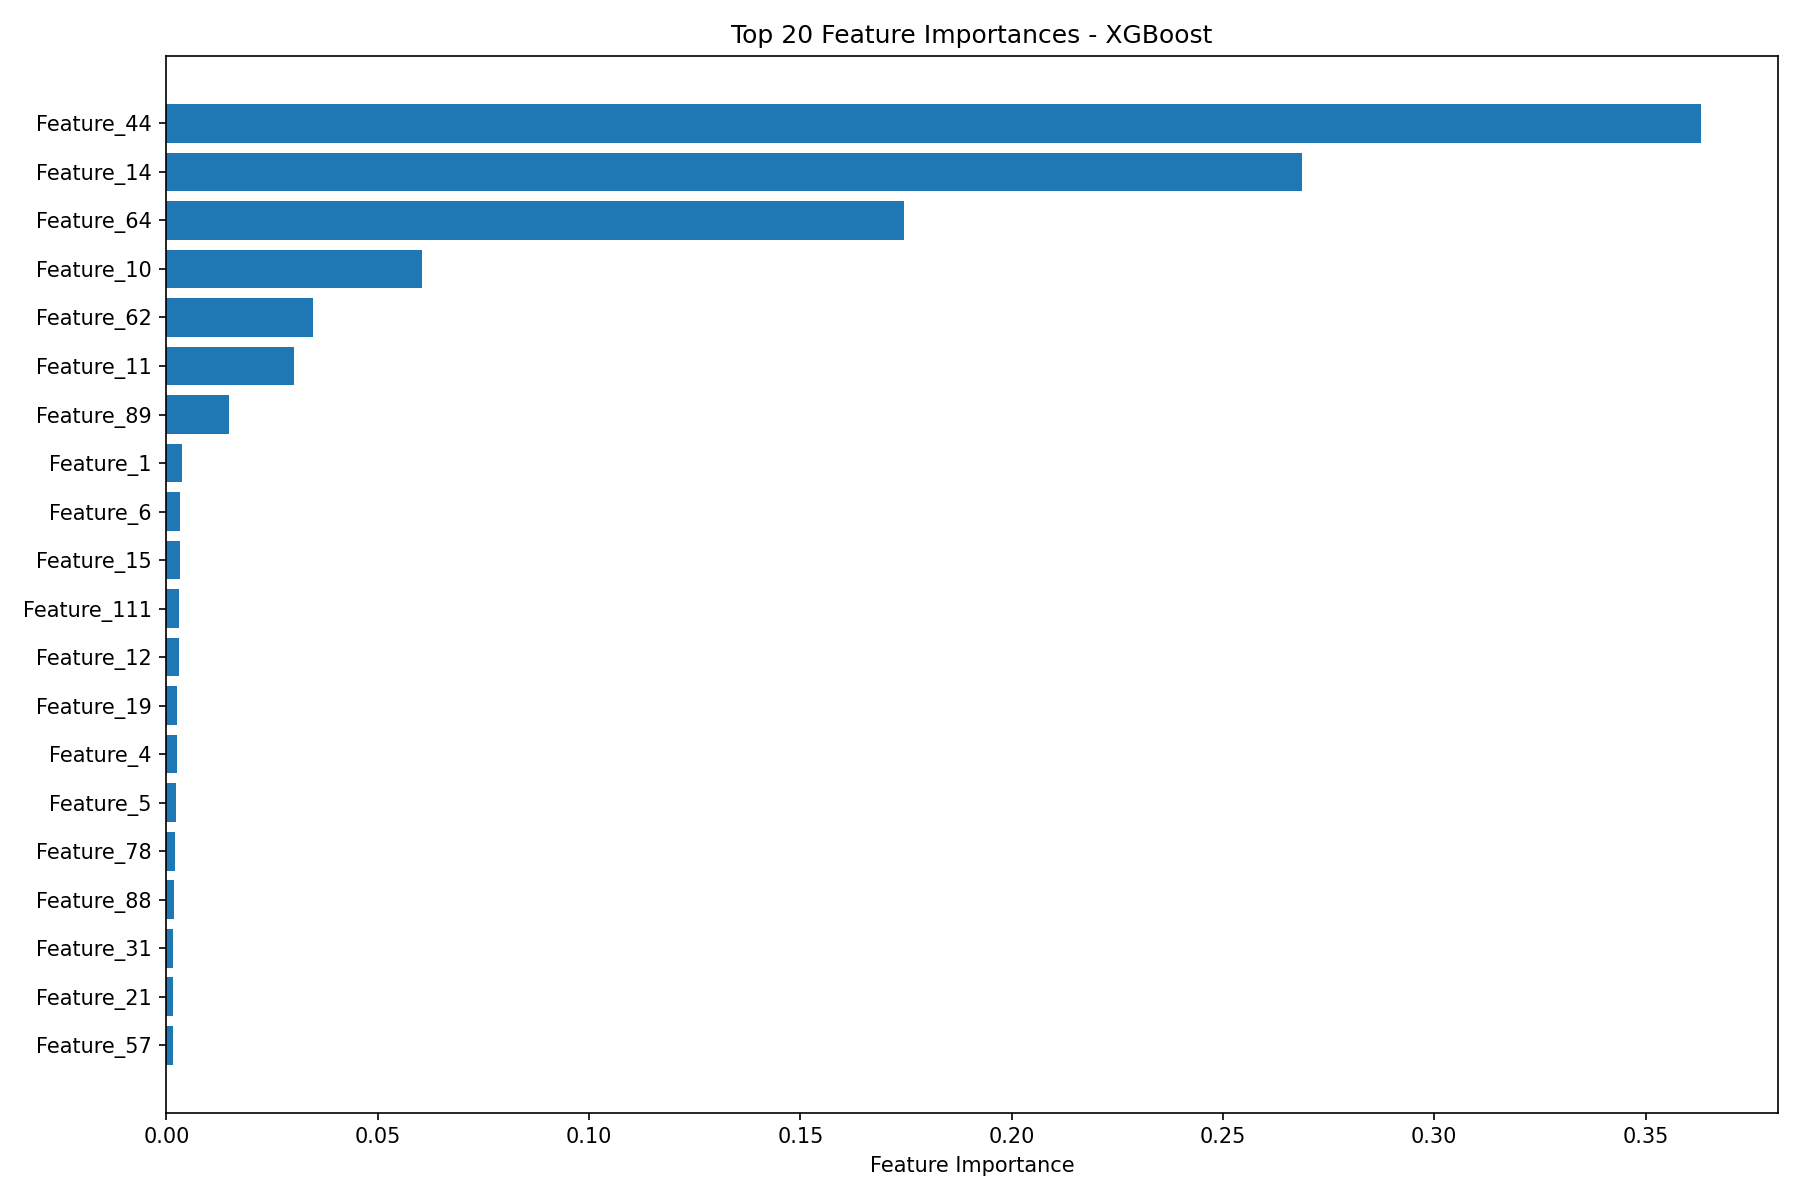
\includegraphics[width=0.95\textwidth]{feature_importance.png}
\caption{Most influential features in the XGBoost churn prediction model.}
\label{fig:feature_importance}
\end{figure}

\subsection{Segment Distribution}

Unlike classification metrics, this visualization focuses on behavioral patterns discovered through segmentation. It presents clustering outcomes from two perspectives:
\begin{itemize}
    \item \textbf{Pie chart}: Customer distribution by segment
    \item \textbf{Bar chart}: Churn rate by segment
\end{itemize}

\begin{figure}[H]
\centering
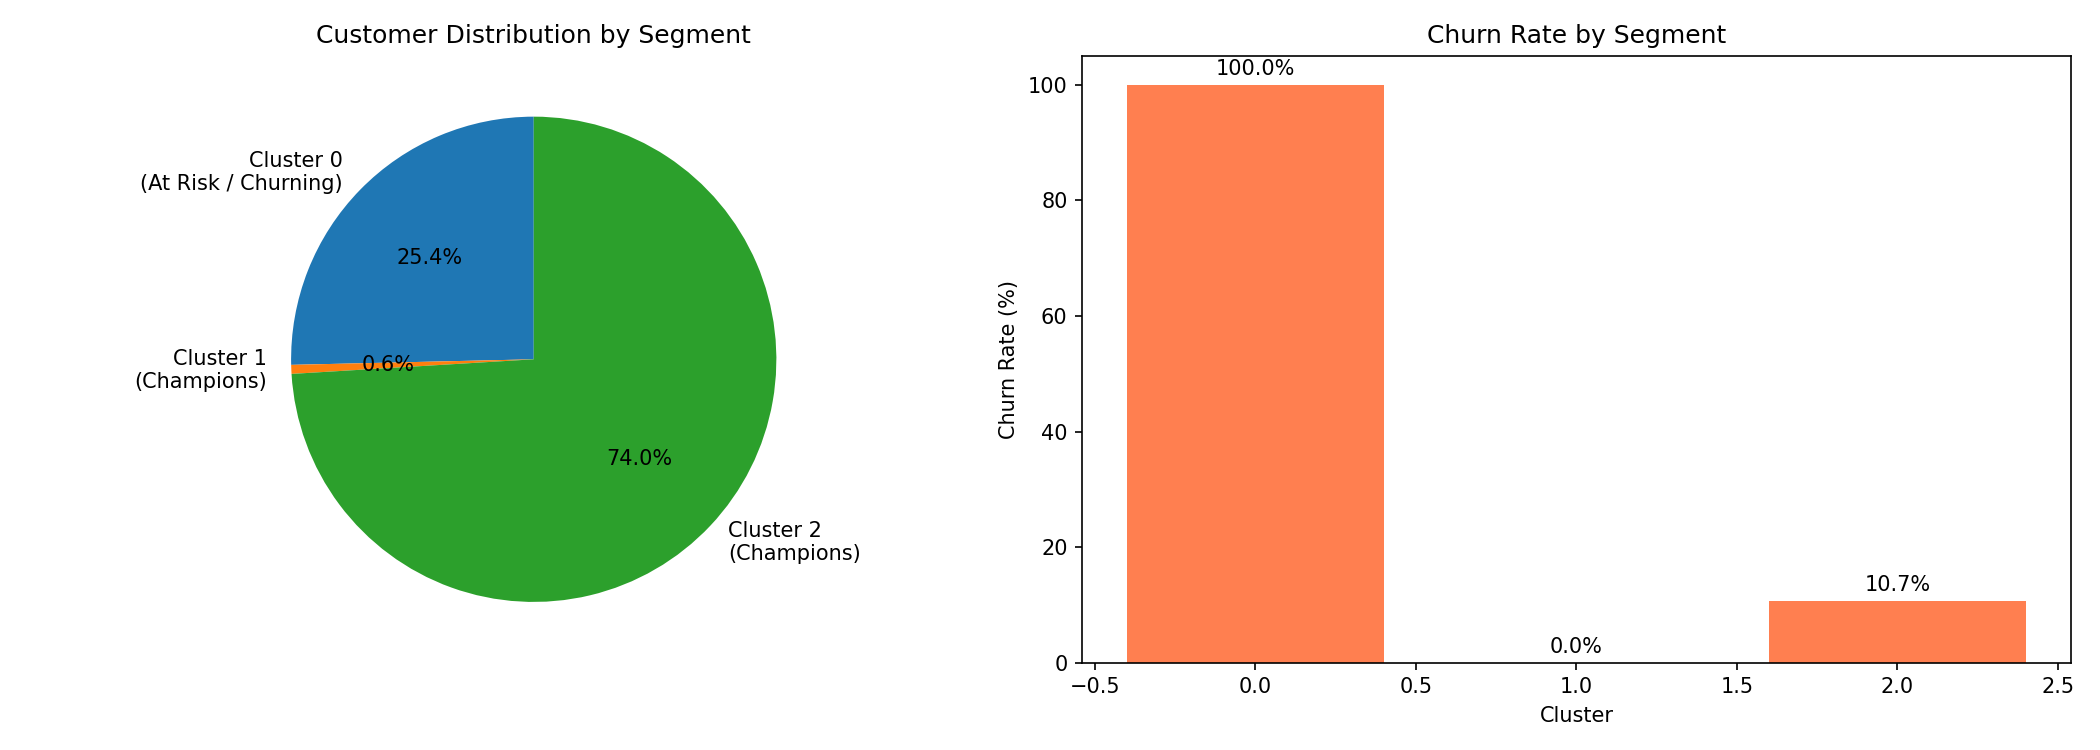
\includegraphics[width=0.95\textwidth]{segment_distribution.png}
\caption{Customer distribution by segment and comparison of associated churn rates.}
\label{fig:segment_distribution}
\end{figure}

\subsection{RFM Profile Heatmap}

To summarize the distinctive characteristics of each segment, a normalized heatmap provides an overview of RFM profiles. It displays a color matrix of normalized RFM values by segment:
\begin{itemize}
    \item Rows: RFM metrics (Recency, Frequency, Monetary)
    \item Columns: Customer segments
    \item Values: Normalized scores between 0 and 1
\end{itemize}

%==============================================================================
\section{Flask Interface Deployment}
%==============================================================================

To complete the deployment phase of the project, we implemented a Flask-based interface that operationalizes the trained churn model and segmentation outputs for end users.

\subsection{Deployment Objective}

The objective of this interface is to transform the analytical pipeline into a usable application where a user can:
\begin{itemize}
    \item Predict churn for a specific customer
    \item Score customers in batch mode from the processed dataset
    \item Interpret results through risk levels, segment assignment, and recommended marketing actions
\end{itemize}

\subsection{Implemented Application Structure}

The deployment layer was organized in the \texttt{src/app/} package:
\begin{itemize}
    \item \texttt{web.py}: Flask routes and request handling
    \item \texttt{services.py}: model loading, inference logic, segmentation enrichment, and summaries
    \item \texttt{templates/}: HTML templates (\texttt{base.html}, \texttt{index.html})
    \item \texttt{static/style.css}: interface styling
\end{itemize}

This structure separates presentation, routing, and business logic to improve maintainability.

\subsection{Functionalities Delivered}

\subsubsection{Single-Customer Prediction}
The interface accepts a \texttt{CustomerID}, retrieves the corresponding record from the processed dataset, and displays:
\begin{itemize}
    \item Churn probability and churn decision
    \item Risk level (Low, Medium, High, Critical)
    \item Segment assignment inferred from RFM values
    \item Segment-specific marketing recommendations and channels
\end{itemize}

\subsubsection{Batch Processing with Controlled Pagination}
The \textit{Process all customers} workflow was optimized for responsiveness:
\begin{itemize}
    \item Only the first 100 customers from \texttt{data/processed/retail\_customers\_cleaned.csv} are scored
    \item Results are sorted by ascending churn priority: Low $\rightarrow$ Medium $\rightarrow$ High $\rightarrow$ Critical
    \item Pagination is applied at 10 rows per page with previous/next navigation
\end{itemize}

\subsubsection{Operational API Endpoints}
In addition to the web interface, lightweight endpoints were exposed:
\begin{itemize}
    \item \texttt{/health}: service health check
    \item \texttt{/api/summary}: model and dataset summary
    \item \texttt{/api/predict}: JSON prediction endpoint
\end{itemize}

\subsection{User Interface Adjustments}

To align the interface with a more professional presentation, the UI was refined with:
\begin{itemize}
    \item Header removal for a cleaner layout
    \item Neutral grayscale palette replacing the previous blue accent
    \item Square/block visual style (no rounded corners)
\end{itemize}

These adjustments improved readability and consistency for report/demo usage.

%==============================================================================
\section{Conclusion}
%==============================================================================

This project delivered a complete customer behavioral analytics solution including:

\begin{enumerate}
    \item \textbf{A robust preprocessing pipeline} handling missing values (KNN for age), anomalous values (sentinel values), and feature engineering (temporal and geographic feature extraction).

    \item \textbf{Rigorous data leakage detection} that led to excluding 4 variables (ChurnRiskCategory, RFMSegment, CustomerType, Recency) that would have artificially inflated model performance.

    \item \textbf{A high-performing churn prediction model} (XGBoost) achieving an F1 score of 98.6\% and ROC-AUC of 99.97\% on the test set.

    \item \textbf{Actionable customer segmentation} identifying three distinct segments with tailored marketing recommendations.
\end{enumerate}

\subsection{Future Work}

Several improvement paths can be considered:
\begin{itemize}
    \item Integrating temporal data for time-series analysis
    \item Building an interactive dashboard for real-time monitoring
    \item Deploying the model through a REST API
    \item Running A/B tests on segment-based marketing recommendations
\end{itemize}

\end{document}
